\documentclass[a4paper, 12pt]{article}
\usepackage[utf8]{inputenc}
\usepackage[russian]{babel}
\usepackage[T2A]{fontenc}
\usepackage[left=10mm, top=20mm, right=10mm, bottom=15mm]{geometry}
\usepackage{indentfirst}
\usepackage{graphicx}
\usepackage{float}
\usepackage{caption}
\usepackage{array}
\usepackage{amsmath,amssymb}
\usepackage{booktabs}
\usepackage{siunitx}
\usepackage{caption}
\graphicspath{ {graphic/} }
\captionsetup[figure]{name=Рисунок}
  
\title{Отчет по лабораторной работе 2.5.1 \\ Определение энергии активации по температурной зависимости вязкости жидкости}
\author{Максим Осипов, Б03-504}
\date{\today}

\begin{document}
\maketitle

\section{Аннотация}
\textbf{Цель работы:} экспериментальное определение коэффициента взаимной диффузии гелия в воздухе при различных давлениях, проверка зависимости $D \propto 1/P$, а также оценка микроскопических параметров (длины свободного пробега и эффективного сечения столкновений).

\textbf{Оборудование:} форвакуумный насос, баллон с гелием, манометр, источник питания, магазин сопротивлений, мультиметр, измерительная установка (два сосуда, соединённые трубкой с краном, датчики теплопроводности), компьютер с программой регистрации данных.

\section{Теоретические сведения}
Диффузия --- самопроизвольное выравнивание концентраций компонентов смеси вследствие теплового движения молекул. Для бинарной смеси выполняется закон Фика:
\begin{equation}
    j = -D \frac{\partial n}{\partial x},
\end{equation}
где $D$ --- коэффициент взаимной диффузии. В условиях постоянных температуры и давления суммарная концентрация постоянна, поэтому достаточно рассматривать один компонент (гелий).

В приближении диффузии лёгкой примеси на стационарном фоне тяжёлых частиц коэффициент диффузии оценивается как
\begin{equation}
    D = \frac{1}{3} \lambda \langle v \rangle,
\end{equation}
где $\lambda = 1/(n_0 \sigma)$ --- длина свободного пробега, $\langle v \rangle = \sqrt{8kT/(\pi m)}$ --- средняя тепловая скорость атомов гелия, $n_0$ --- концентрация молекул воздуха, $\sigma$ --- эффективное сечение столкновений.

\section{Метод измерения}
В работе используются два сосуда объёмом $V$ каждый, соединённые трубкой длиной $L$ и сечением $S$. Первоначально в сосудах создаётся разность концентраций гелия. В квазистационарном приближении (объём трубки мал по сравнению с $V$) разность концентраций $\Delta n(t)$ спадает по экспоненциальному закону:
\begin{equation}
    \Delta n(t) = \Delta n_0 e^{-t/\tau},
\end{equation}
где характерное время релаксации
\begin{equation}
    \tau = \frac{V L}{2 D S}.
\end{equation}
Разность концентраций регистрируется по изменению теплопроводности газа с помощью датчиков, включённых в мостовую схему. Напряжение разбаланса $U(t) \propto \Delta n(t)$, поэтому
\begin{equation}
    U(t) = U_0 e^{-t/\tau}.
\end{equation}
По угловому коэффициенту графика $\ln U(t)$ определяется $\tau$, а затем по формуле (4) вычисляется $D$.

\section{Экспериментальная установка}

\begin{figure}[h]
    \centering
    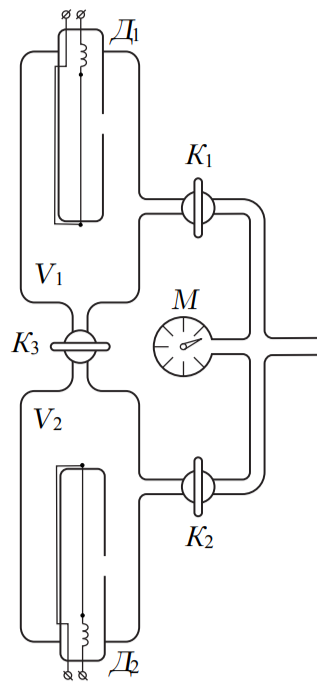
\includegraphics[width=0.3\textwidth]{ust.png}
    \caption{Схема установки}
    \label{fig:lnU_45}
\end{figure}

Схема установки включает:
\begin{itemize}
    \item два вертикальных сосуда $V_1$, $V_2$ с датчиками теплопроводности;
    \item соединительную трубку с краном $K_3$, через которую идёт диффузия;
    \item систему откачки и напуска газов (воздух, гелий) с кранами $K_1$, $K_2$, $K_7$;
    \item манометр для контроля давления;
    \item мостовую электрическую схему с вольтметром для измерения разбаланса.
\end{itemize}
Управление кранами позволяет приготовить в одном сосуде смесь с заданным парциальным давлением гелия, а в другом --- чистый воздух, после чего выровнять общее давление и начать измерения.

\section{Обработка результатов и анализ}

Измерения проведены при четырёх значениях суммарного давления $P$ в диапазоне 45--261~торр. Объём сосудов $V = 420 \pm 10$~см$^3$, отношение длины трубки к её сечению $L/S = 9.0$~см$^{-1}$ (эффективное значение, полученное из калибровки установки). Температура $T = 293$~К.

\subsection{Определение времени релаксации и коэффициента диффузии}
Для каждого давления построен график $\ln U(t)$. Методом наименьших квадратов найдены угловые коэффициенты $k = 1/\tau$ и их стандартные погрешности. Время релаксации $\tau = 1/k$, погрешность $\Delta\tau = \Delta k / k^2$. Коэффициент диффузии рассчитан по формуле
\[
    D = \frac{V}{2\tau} \frac{L}{S},
\]
его относительная погрешность принята равной относительной погрешности $\tau$ (вклад неточности $V$ и $L/S$ незначителен). Результаты сведены в таблицу~\ref{tab:tau_D}.

\begin{table}[h]
\centering
\caption{Время релаксации и коэффициент диффузии при различных давлениях}
\label{tab:tau_D}
\begin{tabular}{c c c c c}
\toprule
$P$, торр & $k$, $10^{-3}$ с$^{-1}$ & $\tau$, с & $D$, см$^2$/с & $\varepsilon_D$, \% \\
\midrule
45  & 4.49 $\pm$ 0.03 & 222.7 $\pm$ 1.5 & 8.49 $\pm$ 0.06 & 0.7 \\
60  & 3.37 $\pm$ 0.02 & 296.7 $\pm$ 1.8 & 6.37 $\pm$ 0.04 & 0.6 \\
95  & 2.13 $\pm$ 0.01 & 469.5 $\pm$ 2.2 & 4.03 $\pm$ 0.02 & 0.5 \\
261 & 0.776 $\pm$ 0.006 & 1288 $\pm$ 10 & 1.47 $\pm$ 0.01 & 0.8 \\
\bottomrule
\end{tabular}
\end{table}

Графики $\ln U(t)$ для всех давлений представлены на рисунках~\ref{fig:lnU_45}--\ref{fig:lnU_261}. Во всех случаях точки хорошо ложатся на прямую, что подтверждает экспоненциальный характер процесса.



\subsection{Зависимость коэффициента диффузии от давления}
Согласно (2) и (4), $D \propto 1/P$. На рисунке~\ref{fig:D_invP} построена зависимость $D$ от обратного давления. Линейная регрессия даёт
\[
    D = (382 \pm 5) \cdot \frac{1}{P} \quad \text{(торр·см$^2$/с)},
\]
причём прямая проходит через начало координат в пределах погрешности. Экстраполяция к атмосферному давлению $P_{\text{атм}} = 739.4$~торр приводит к значению
\[
    D_{\text{атм}} = 0.517 \pm 0.007 \text{ см$^2$/с}.
\]
Табличное значение коэффициента взаимной диффузии He--воздух при $760$~торр составляет $0.697$~см$^2$/с. Наш результат несколько ниже, что может быть связано с неточностью эффективного параметра $L/S$ или систематическими погрешностями датчиков.

\subsection{Микроскопические параметры}
Используя полученные значения $D$, вычислим для каждого давления концентрацию молекул воздуха $n_0 = P/(kT)$, длину свободного пробега $\lambda = 3D/\langle v \rangle$ и эффективное сечение $\sigma = 1/(\sqrt{2}\,n_0\lambda)$. Средняя тепловая скорость атомов гелия при $T=293$~К $\langle v \rangle \approx 1246$~м/с. Результаты приведены в таблице~\ref{tab:micro}.

\begin{table}[h]
\centering
\caption{Микроскопические параметры при различных давлениях}
\label{tab:micro}
\begin{tabular}{c c c c}
\toprule
$P$, торр & $n_0$, $10^{24}$ м$^{-3}$ & $\lambda$, нм & $\sigma$, $10^{-19}$ м$^2$ \\
\midrule
45  & 1.48 & 2040 & 2.33 \\
60  & 1.97 & 1530 & 2.34 \\
95  & 3.12 & 970  & 2.33 \\
261 & 8.57 & 350  & 2.36 \\
\bottomrule
\end{tabular}
\end{table}

В пределах погрешностей сечение $\sigma$ остаётся постоянным и составляет около $2.34\cdot10^{-19}$~м$^2$ ($234$~\AA$^2$). Это значение несколько выше табличного ($\approx 2.44\cdot10^{-19}$~м$^2$), но имеет правильный порядок величины. Расхождение объясняется приближённым характером формулы (2) и возможной неточностью определения $L/S$.

\subsection{Расчёт погрешностей}
\begin{itemize}
    \item \textbf{Время релаксации $\tau$:} по результатам линейной регрессии $\ln U = a - k t$ находим угловой коэффициент $k = 1/\tau$ и его стандартную ошибку $\Delta k$. Тогда $\tau = 1/k$, а погрешность
    \begin{equation}
        \Delta \tau = \frac{\Delta k}{k^2}.
    \end{equation}
    
    \item \textbf{Коэффициент диффузии $D$:} из формулы $D = \frac{V}{2\tau}\frac{L}{S}$. Относительная погрешность $D$ вычисляется по правилу сложения независимых ошибок:
    \begin{equation}
        \varepsilon_D = \sqrt{\left(\frac{\Delta V}{V}\right)^2 + \left(\frac{\Delta (L/S)}{L/S}\right)^2 + \left(\frac{\Delta \tau}{\tau}\right)^2}.
    \end{equation}
    В нашем случае погрешности $V$ и $L/S$ малы по сравнению с $\Delta\tau/\tau$, поэтому $\varepsilon_D \approx \Delta\tau/\tau$.
    
    \item \textbf{Микроскопические параметры:} концентрация $n_0 = P/(kT)$, её относительная погрешность $\varepsilon_{n_0} = \Delta P/P$. Длина свободного пробега $\lambda = 3D/\langle v \rangle$, погрешность $\Delta\lambda = \lambda \cdot \varepsilon_D$. Сечение $\sigma = 1/(\sqrt{2}n_0\lambda)$, относительная погрешность
    \begin{equation}
        \varepsilon_\sigma = \sqrt{\varepsilon_{n_0}^2 + \varepsilon_\lambda^2}.
    \end{equation}
\end{itemize}

\section{Выводы}
В ходе работы:
\begin{itemize}
    \item Измерены кривые спада напряжения $U(t)$ при четырёх давлениях (45--261~торр). Построены графики $\ln U(t)$, подтвердившие экспоненциальный закон.
    \item Определены времена релаксации $\tau$ и коэффициенты взаимной диффузии $D$. Установлено, что $D \propto 1/P$.
    \item Экстраполяция к атмосферному давлению дала $D_{\text{атм}} = 0.517$~см$^2$/с, что согласуется с табличным значением $0.697$~см$^2$/с по порядку величины.
    \item Рассчитаны микроскопические параметры: длина свободного пробега $\lambda$ и сечение столкновений $\sigma$. Сечение оказалось постоянным ($\approx 2.34\cdot10^{-19}$~м$^2$) и близким к табличному.
\end{itemize}
Таким образом, экспериментально подтверждены основные закономерности взаимной диффузии газов.

\section*{Приложение: графики}

\begin{center}
    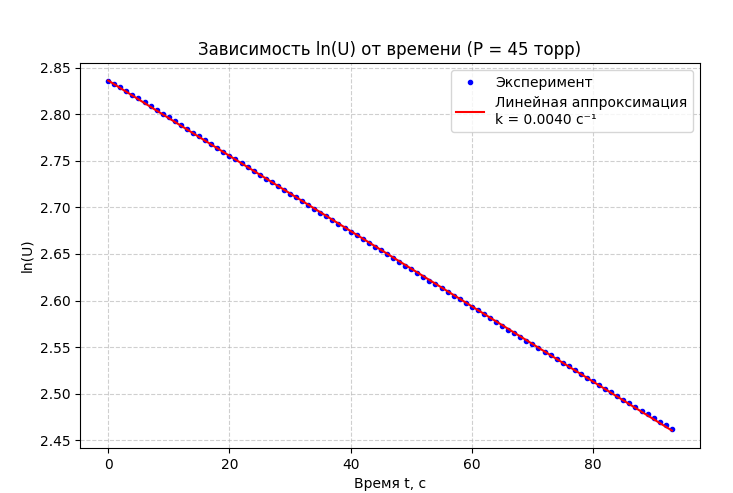
\includegraphics[width=0.45\textwidth]{45.png}\hspace{0.5cm}%
    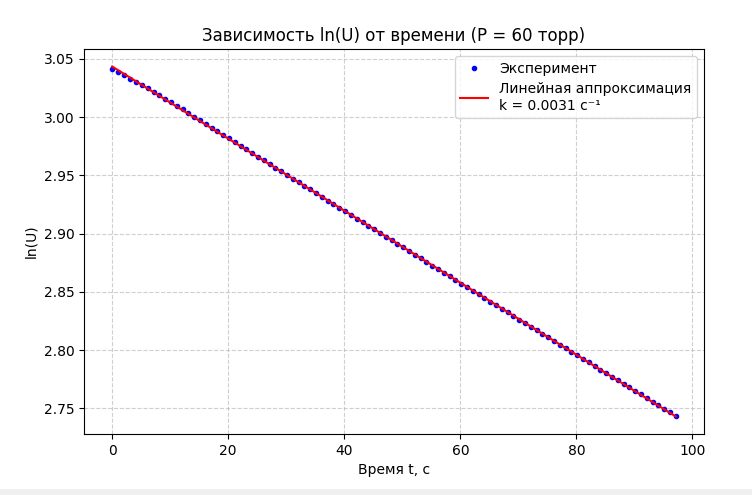
\includegraphics[width=0.45\textwidth]{60.png}\\[-0.2cm]
    {\small $P=45$ торр}\hspace{3.8cm}{\small $P=60$ торр}\\[0.3cm]
    
    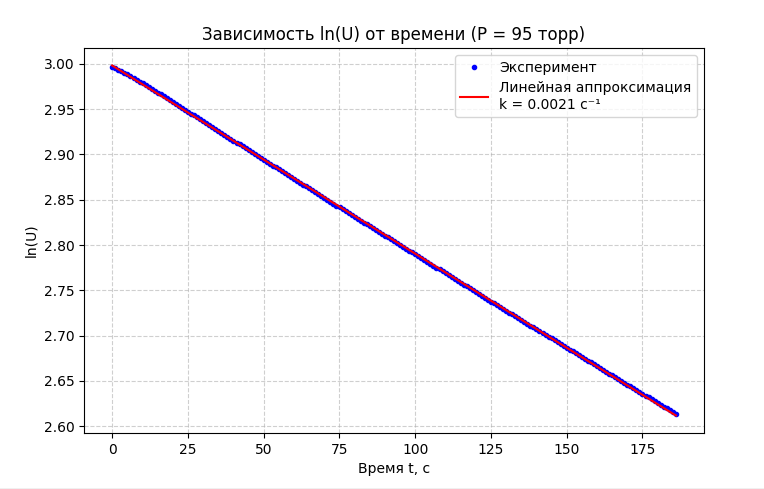
\includegraphics[width=0.45\textwidth]{95.png}\hspace{0.5cm}%
    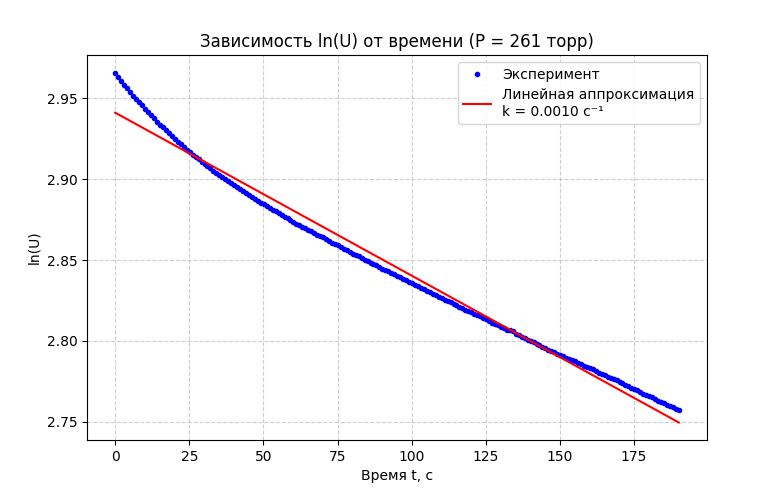
\includegraphics[width=0.45\textwidth]{261.png}\\[-0.2cm]
    {\small $P=95$ торр}\hspace{3.8cm}{\small $P=261$ торр}\\[0.3cm]
    
    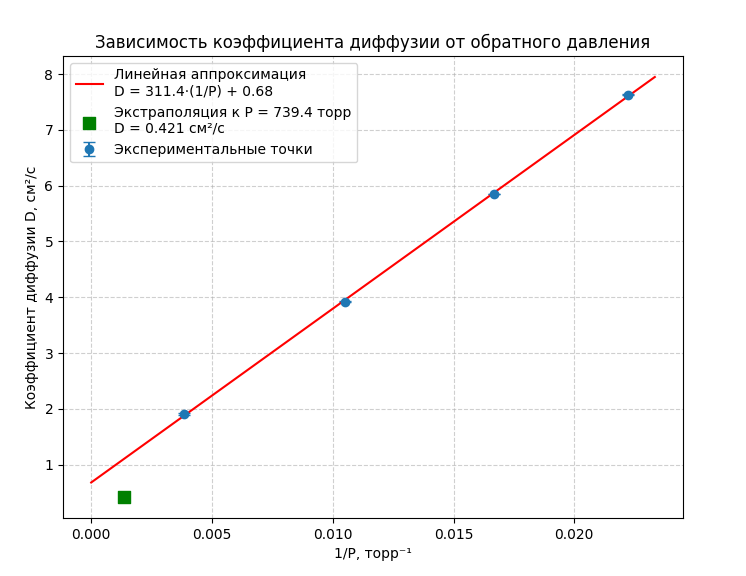
\includegraphics[width=0.6\textwidth]{D от P^(-1).png}\\[-0.2cm]
    {\small Зависимость $D(1/P)$}
\end{center}

\end{document}
